\documentclass[a4paper,12pt]{article}

%\begin{figure}[htp]
%    \centering
%    \includegraphics[width=0.75\textwidth]{}
%\end{figure}

%%%%%%%%%%%%%%%%%%%%
%%%%  PREAMBLE  %%%%
%%%%%%%%%%%%%%%%%%%%
\usepackage{float}
\usepackage[T1]{fontenc}
\usepackage[utf8]{inputenc}

\usepackage[english,italian]{babel}
\usepackage{graphicx}     % Per includere immagini
\usepackage{subcaption}   % Per utilizzare subfigure
\usepackage{hyperref}
\hypersetup{hidelinks}

\usepackage[margin=2.5cm]{geometry}
\usepackage{minipage-marginpar}
\usepackage{fancyhdr}
\usepackage[bottom]{footmisc}
\usepackage{lastpage}

\usepackage{enumitem}
\usepackage{tabularx}

\usepackage{graphicx}

\setlength{\parindent}{0em}
\setlength{\parskip}{1em}

\fancyhead[L]{\leftmark}
\fancyhead[R]{\shortstack[r]{Versione documento: 0.01 \\ Gruppo: G24}}

\fancyfoot[C]{}
\fancyfoot[R]{\thepage/\pageref{LastPage}}

\renewcommand{\headrulewidth}{2pt}
\renewcommand{\headruleskip}{3pt}
\setlength{\headheight}{30pt}

\renewcommand{\footrulewidth}{2pt}

\setlist[itemize]{itemsep=0.25em,topsep=0pt}
\setlist[enumerate]{itemsep=0.25em,topsep=0pt,align=left}

%%%%%%%%%%%%%%%%%%%%
%%%%  DOCUMENT  %%%%
%%%%%%%%%%%%%%%%%%%%

\title{}
\author{Gruppo G24}

\begin{document}

\pagestyle{empty}

\begin{center}

    \vspace{2 cm}

    \begin{tabular*}{\textwidth}{ c @{\extracolsep{\fill}} c }
        
\includegraphics[width=0.3\textwidth]{marchio_unitrento.pdf} & \shortstack{\Large{Dipartimento di Ingegneria} \\ \Large{e Scienza dell'Informazione}}
    \end{tabular*}

    \vspace{5 cm} 
  
    \Huge \textbf{Ingegneria del software\\}
  
    \vspace{1.5 cm} 
    \Large\textsc{Documento dei requisiti\\} 
    \vspace{3 cm} 
    \Huge\textsc{Mountain Wonders\\}
    \Large{Gruppo G24}
  
    \vspace{2 cm} 
  
    \Large{Anno accademico 2023/2024}
\end{center}

\newpage
\tableofcontents

\pagestyle{fancy}
\newpage
\section{Scopo del documento}

Il presente documento riporta l’analisi dei requisiti di sistema del progetto MountainWonders. Lo scopo di questo di questo documento è quello di:
\begin{itemize}
    \item presentare gli obiettivi del progetto;
    \item descrivere i requisiti funzionali;
    \item elencare i requisiti non funzionali;
    \item presentare il front-end del progetto;
    \item descrivere il back-end del progetto.
\end{itemize}

\section{Obiettivi del progetto}

Questo progetto ha l’obiettivo di realizzare una piattaforma web per la visualizzazione di rifugi e punti di spicco del Trentino - Alto Adige. In particolare si concentrerà sulla loro catalogazione e la possibilità da parte degli utenti di valutare determinati parametri di essi. 
Nello specifico l'applicazione sarà in grado di:

\begin{itemize}
    \item Effettuare la registrazione di nuovi utenti tramite l’inserimento delle informazioni necessarie per creare un account, come nome, indirizzo email e password. 

    \item Permettere ad un utente di effettuare l’accesso al proprio account tramite la verifica delle credenziali.

    \item Permettere ad un utente registrato di poter inserire un rifugio o punti di spicco (fiumi, laghi, viste particolari) con l’aggiunta di foto.

    \item Permettere ad un utente registrato di inserire recensioni con determinati tag: Generale, vista, laghi-fiumi(se presente), animali, attrazioni (parchi, mostre, …).
    
    \item Permettere ad un utente, registrato o non, di effettuare una ricerca tra i percorsi disponibili in base ai filtri o al nome della montagna.
\end{itemize}
\newpage

\section{Requisiti funzionali}

Vengono elencati di seguito i requisiti funzionali, ossia quei requisiti legati alle funzionalità del sistema.



\subsection*{RF1 Registrazione}
Il sito dovrà presentare una pagina dedicata alla registrazione di un nuovo utente che visita il sito. Per effettuare la registrazione sarà necessaria una email valida e una password. Per completare la registrazione sarà inoltre necessaria la verifica tramite un'email di conferma.
\begin{enumerate} [leftmargin=40pt]
    \item Nel caso in cui i dati inseriti non siano validi, l'applicazione provvederà a mostrare un messaggio di errore per informare l'utente. 
\end{enumerate}


\subsection*{RF2 Login}
 Il sito presenterà una pagina dedicata all’accesso tramite credenziali (email-password) precedentemente registrate (RF1).
 Il sito web provvede quindi a verificare la correttezza dei dati inseriti per permettere all'utente di accedere all'area riservata.
 \begin{enumerate} [leftmargin=40pt]
    \item Qualora le credenziali siano errate, verrà mostrato un messaggio di errore per avvisare l'utente.
\end{enumerate}


\subsection*{RF3 Recupero password}
La schermata di login dovrà presentare un link che permetta il reindirizzamento alla pagina "Recupera password", dove sarà possibile recuperare la propria password tramite una email.
 \begin{enumerate} [leftmargin=40pt]
    \item Qualora la mail non venga trovata tra le credenziali degli utenti, verrà mostrato un messaggio di errore. 
\end{enumerate}


\subsection*{RF4 Account Amministratore}
Nel sito web sarà presente un account amministratore, che avrà accesso a funzionalità privilegiate e poteri estesi all'interno del sito.\\
L'account admin sarà fondamentale per la gestione e il controllo completo del sito web. Di seguito sono elencate le principali caratteristiche e le responsabilità dell'account admin:
 \begin{itemize} [itemindent=0.5cm]
     \item eliminare utenti;
     \item eliminare una recensione;
 \end{itemize}


\subsection*{RF5 Eliminare utenti - Admin}
Qualora un utente non rispetti le norme del sito (RNF7) o voglia eliminare il proprio account, l'applicazione permetterà all'account amministrazione di eliminare l'account con i relativi dati personali inseriti al momento della registrazione.


\subsection*{RF6 Eliminare una recensione - Admin}
Il sito permetterà all'amministratore di eliminare una recensione nel caso in cui questa non rispetti le norme del sito (RNF7). L'operazione verrà notificata all'utente e nel caso in cui l'evento si ripeta eliminerà definitivamente l'account registrato (RF7). 


\subsection*{RF7 Account registrato}
 Il sito presenterà una sezione per la visualizzazione dell'account registrato, dove sarà possibile:
 \begin{enumerate} [leftmargin=40pt]
     \item visionare i dati personali
     \item visionare le recensioni effettuate
     \item cambiare la password del proprio account
     \item chiedere l'eliminazione del proprio account
 \end{enumerate}

 \subsection*{RF8 Account anonimo}
 La pagina permetterà anche di gestire un utente anonimo, ossia un utente che non ha effettuato la registrazione al sito.\\
 Questo avrà funzionalità più limitate rispetto ad un utente registrato, infatti l'applicazione web gli permetterà di:
 \begin{enumerate} [leftmargin=40pt]
  \item visualizzare l'elenco dei rifugi e luoghi di spicco
  \item visualizzare l'elenco delle montagne
  \item visionare eventuali recensioni relative ad un rifugio o ad una montagna
\end{enumerate}
 
 

 
\subsection*{RF9 Dati personali}
L'applicazione offrirà agli utenti la possibilità di eseguire diverse operazioni relative alla gestione del proprio profilo personale. Le principali operazioni sono: 

\begin{enumerate} [leftmargin=40pt]
  \item \textbf{Caricare una foto profilo:} L'applicazione permetterà agli utenti di selezionare e caricare un'immagine che rappresenti il loro profilo. Questa foto sarà visibile agli altri utenti e contribuirà a personalizzare il loro profilo.

  \item \textbf{Modificare la foto profilo:} Il sito permetterà, oltre al caricamento iniziale, di apportare modifiche alla foto del profilo quando lo si desidera. 

  \item \textbf{Visualizzare dati personali:} In questa sezione, gli utenti avranno accesso ai propri dati personali registrati nell'applicazione. Potranno visualizzare informazioni quali nome, cognome, data di nascita, indirizzo email e altre informazioni pertinenti.

  \item \textbf{Aggiornare dati personali:} L'applicazione permetterà inoltre di apportare modifiche e aggiornamenti a tali dati, garantendo che le informazioni del proprio account siano sempre accurate e aggiornate.
\end{enumerate}


\subsection*{RF10 Cambio password}
Il sito, tramite l’apposita sezione nel proprio account (FR8), permetterà all’utente di cambiare la propria password utilizzando l’email ricevuta per confermare l'operazione.


\subsection*{RF11 Elimina account}
Nell’apposita sezione, l'applicazione consentirà all'utente di effettuare la cancellazione dell'account grazie alla quale (previa conferma via email) sarà possibile eliminare le proprie informazioni personali.


\subsection*{RF12 Recensioni}
L'applicazione deve permettere ad un utente registrato di poter recensire ciascun rifugio o luogo di spicco.\\
In questo modo, il rating della recensione potrà poi essere usato nell'area di ricerca, per fornire risultati specifici all'utente che ha effettuato la ricerca. 


\subsection*{RF13  Recensioni effettuate}
La web app darà la possibilità ad un utente che ha effettuato l'accesso al proprio account(RF8) di vedere tutte le recensioni da lui effettuate, elencate in ordine di data di pubblicazione.


\subsection*{RF14 Modifica-Elimina recensione}
Recandosi nella pagina in cui si è effettuata una recensione (RF12) o nella sezione del proprio account in cui vengono visualizzate le proprie recensioni effettuate(RF13), l'applicazione permetterà all'utente di modificare o eliminare una recensione precedentemente fatta.\\
Una volta che l'utente ha effettuato l'accesso con successo al proprio account, il sito garantirà un accesso alla sezione dedicata alle recensioni da lui create. Questa sezione mostrerà in modo chiaro e organizzato l'elenco completo delle recensioni precedentemente inviate dall'utente, consentendogli di accedervi con facilità.


\subsection*{RF15 Ricerca}
Gli utenti avranno la possibilità di effettuare la ricerca di rifugi o luoghi di spicco grazie all’utilizzo di un’apposita barra di ricerca.\\
Durante l'operazione di ricerca di un rifugio o di un luogo di spicco, l'applicazione consentirà all'utente di raffinare la sua ricerca tramite l'uso di filtri.\\
Questi filtri rappresentano una serie di criteri che l'utente può selezionare per fare in modo che la ricerca produca dei risultati specifici.
Tali filtri potrebbero essere diversi parametri quali la posizione geografica, la distanza, le valutazioni degli altri utenti, la difficoltà.


\subsection*{RF16 Pagine di visualizzazione}
Il sito web permetterà ad un utente registrato e non registrato di visualizzare l'elenco dei rifugi e luoghi di spicco.\\
Inoltre, tramite un'apposita pagina, l'applicazione web permetterà di visionare i dettagli di un rifugio o di un luogo di spicco.\\
Il sistema fornirà un'ulteriore pagina per la visualizzazione delle montagne.


\subsection*{RF17 Aggiungere rifugio o luogo di spicco}
Il sito permetterà agli utenti di contribuire attivamente all'espansione del database, consentendo loro di aggiungere nuovi rifugi o luoghi di notevole interesse. Questa funzionalità svolge un ruolo fondamentale nel mantenere il sito costantemente arricchito e aggiornato, garantendo che sia una risorsa informativa completa e sempre in evoluzione. Con questa possibilità, gli utenti possono condividere le loro esperienze e conoscenze personali sulla montagna.

\subsection*{RF18 Supporto}
Il sito web deve includere una pagina dedicata al supporto, fornendo agli utenti un mezzo efficace per richiedere assistenza o informazioni aggiuntive. Le richieste di supporto effettuate tramite questa pagina verranno automaticamente inoltrate all'amministratore (RF4).

\subsection*{RF19 Cambio lingua}
Il sito web deve offrire un menu o un'opzione chiaramente visibile nella parte superiore facilmente accessibile, che consenta agli utenti di selezionare la lingua di loro preferenza. Questo menu deve elencare tutte le lingue supportate.

\newpage
\section{Requisiti non funzionali}

Vengono di seguito elencati e descritti i requisiti non funzionali del progetto. Ciascun requisito diversamente dai requisiti funzionali è legato alle performance.

\subsection*{RNF1 Sicurezza}
\begin{enumerate}[label = \alph*]
    \item Le sezioni dedicate agli utenti registrati devono essere protette da accessi non autorizzati, tramite l’utilizzo di username e password. 
    La password deve rispettare determinati criteri di sicurezza, quali: 
        \begin{itemize}
            \item Una lunghezza minima di 8 caratteri
            \item Lettere sia maiuscole che minuscole
            \item Presenza di almeno un carattere speciale (\&, £, \$, \#, ...)
            \item Presenza di almeno un numero 
        \end{itemize}
    \item Tutti i dati sensibili degli utenti, come informazioni personali e password, saranno crittografati sia in transito che a riposo, ossia quando il dato non viene utilizzato per l'accesso. Saranno implementati protocolli di crittografia standard del settore come TLS/SSL.
\end{enumerate}


\subsection*{RNF2 Performance}
Il sito deve essere in grado di gestire il numero richiesto di utenti senza alcun degrado delle prestazioni. Deve essere inoltre veloce e rendere gradibile la navigazione ad un utente mobile, di conseguenza il tempo di risposta dopo un'operazione dell'utente sarà di massimo 2 secondi. \footnote{"Se il caricamento di un sito Web richiede molto tempo, ciò può avere effetti negativi sull'esperienza dell'utente, sul traffico del sito e sulla SEO (Search Engine Optimization). I siti Web ottimizzati per le prestazioni hanno un vantaggio rispetto ai siti Web lenti."    Cloudflare }


\subsection*{RNF3 Compatibilità}
Il sito web dovrà essere compatibile con le ultime versioni dei seguenti browser e dispositivi:
\begin{itemize}
    \item Browser desktop: Google Chrome, Mozilla Firefox, Microsoft Edge, Safari.
    \item Browser mobile: Safari su iOS, Google Chrome su Android.
\end{itemize}


\subsection*{RNF4 Affidabilità e disponibilità}
Per poter rendere affidabile la web app, i dati inseriti dagli utenti verranno salvati all’interno di un database. Su questi verranno effettuati backup periodici per poter eventualmente recuperare i dati in caso di guasti del sistema o di attacchi informatici.


\subsection*{RNF5 Usabilità}
Il sito web deve essere progettato in modo tale da risultare intuitivo e accessibile, garantendo una facile fruibilità per un pubblico ampio, composto principalmente da individui con un'età compresa tra i 15 e i 50 anni.\\
Questo pubblico variegato potrà accedere e utilizzare il sito sia tramite dispositivi mobili come smartphone e tablet, sia attraverso computer desktop e portatili, al fine di massimizzare la sua adozione e utilizzo in modo versatile e inclusivo.

% \subsection*{RNF6 Lingua}
% Il sito web deve fornire agli utenti la possibilità di cambiare la lingua % dell'interfaccia in modo tale da renderlo più accessibile a persone che parlano lingue diverse \textbf{(RFX)}.\\
%Questa funzionalità è essenziale per garantire una migliore esperienza utente e per raggiungere un pubblico più ampio e diversificato.


\subsection*{RNF6 Norme recensioni}
Per garantire un ambiente informativo, costruttivo e rispettoso, abbiamo stabilito le seguenti linee guida per le recensioni degli utenti:
\begin{itemize}
    \item Le recensioni dovrebbero essere pertinenti a quanto contenuto all'interno della pagina visualizzata
    \item Non inserire commenti offensivi, linguaggio volgare, discriminazione, insulti o minacce verso individui o gruppi.\\
    In caso l'utente admin trovi recensioni non adeguate, provvederà a cancellarla.
    \item La pubblicazione ripetuta di contenuti simili o allo scopo di promuovere un'agenda personale non sarà consentito.
\end{itemize}

\subsection*{RNF7 Gestione delle immagini}
Le immagini devono essere ottimizzate per ridurre i tempi di caricamento e migliorare le prestazioni. Se non gestite correttamente, le immagini possono rallentare significativamente il caricamento del sito e avere un impatto negativo sull'esperienza dell'utente.



\subsection*{RNF8 Privacy}
Il sito web dovrà essere conforme alle seguenti normative e regolamenti:
\begin{itemize}
    \item GDPR (General Data Protection Regulation): il sito raccoglierà e tratterà dati personali degli utenti, nome, cognome, data di nascita, foto dell'utente e email. Saranno forniti avvisi chiari sulla privacy e acquisiti consensi espliciti per la raccolta e l'uso dei dati.
    \item Leggi sul copyright: sarà rispettato il copyright per tutti i contenuti utilizzati sul sito, evitando l'uso non autorizzato di testi, immagini e altri materiali protetti.
    \item COPPA (Children's Online Privacy Protection Act): il sito effettuerà un controllo dell'età dell'utente che si registra, impedendo la registrazione ai minori di 13 anni.
\end{itemize}


\subsection*{RNF9 Aggiornamenti} 
Il sito web sarà progettato e sviluppato con una solida architettura e un'infrastruttura scalabile al fine di garantire la sua capacità di supportare senza problemi eventuali futuri aggiornamenti. Questi aggiornamenti potrebbero essere di natura diversa, tra cui la risoluzione di problemi, l'aggiunta di nuove funzionalità e il miglioramento complessivo dell'esperienza dell'utente.


\newpage
\section{Front-end}
Verranno mostrate di seguito le interfacce delle pagine web con relative descrizioni.
\subsection*{FE1 Homepage}
\begin{figure}[ht]
   \centering
    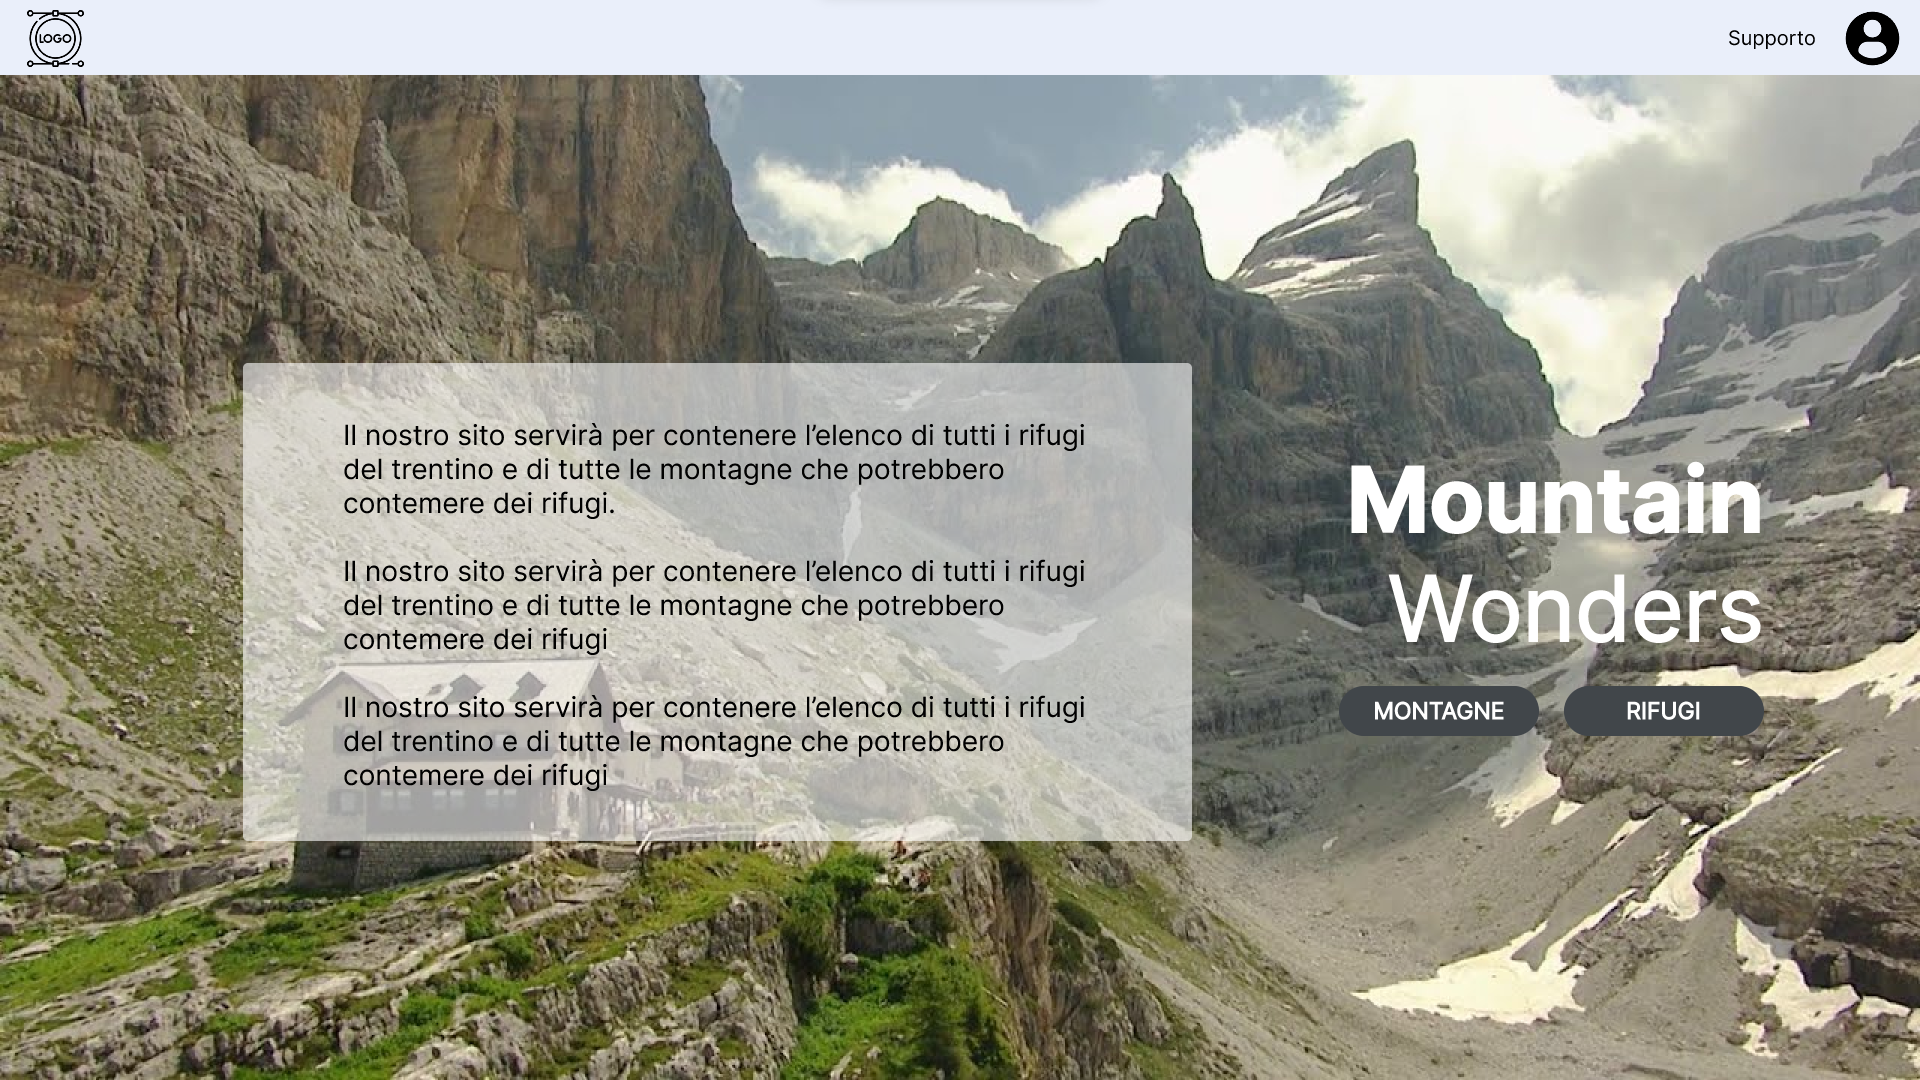
\includegraphics[width=0.6\textwidth]{img/Homepage.png}
    \caption{Homepage}
\end{figure}
Questa sarà la web page principale, da cui sarà possibile recarsi nelle seguenti pagine:
\begin{itemize}
    \item Profilo (RF4, nella barra di navigazione in alto a destra)
    \item Pagina delle montagne (sotto il nome del sito)
    \item Pagina rifugi (sotto il nome del sito)
\end{itemize}


\subsection*{FE2 Sign-up page}
\begin{figure}[H]
  \begin{subfigure}{0.49\textwidth}
    \centering
    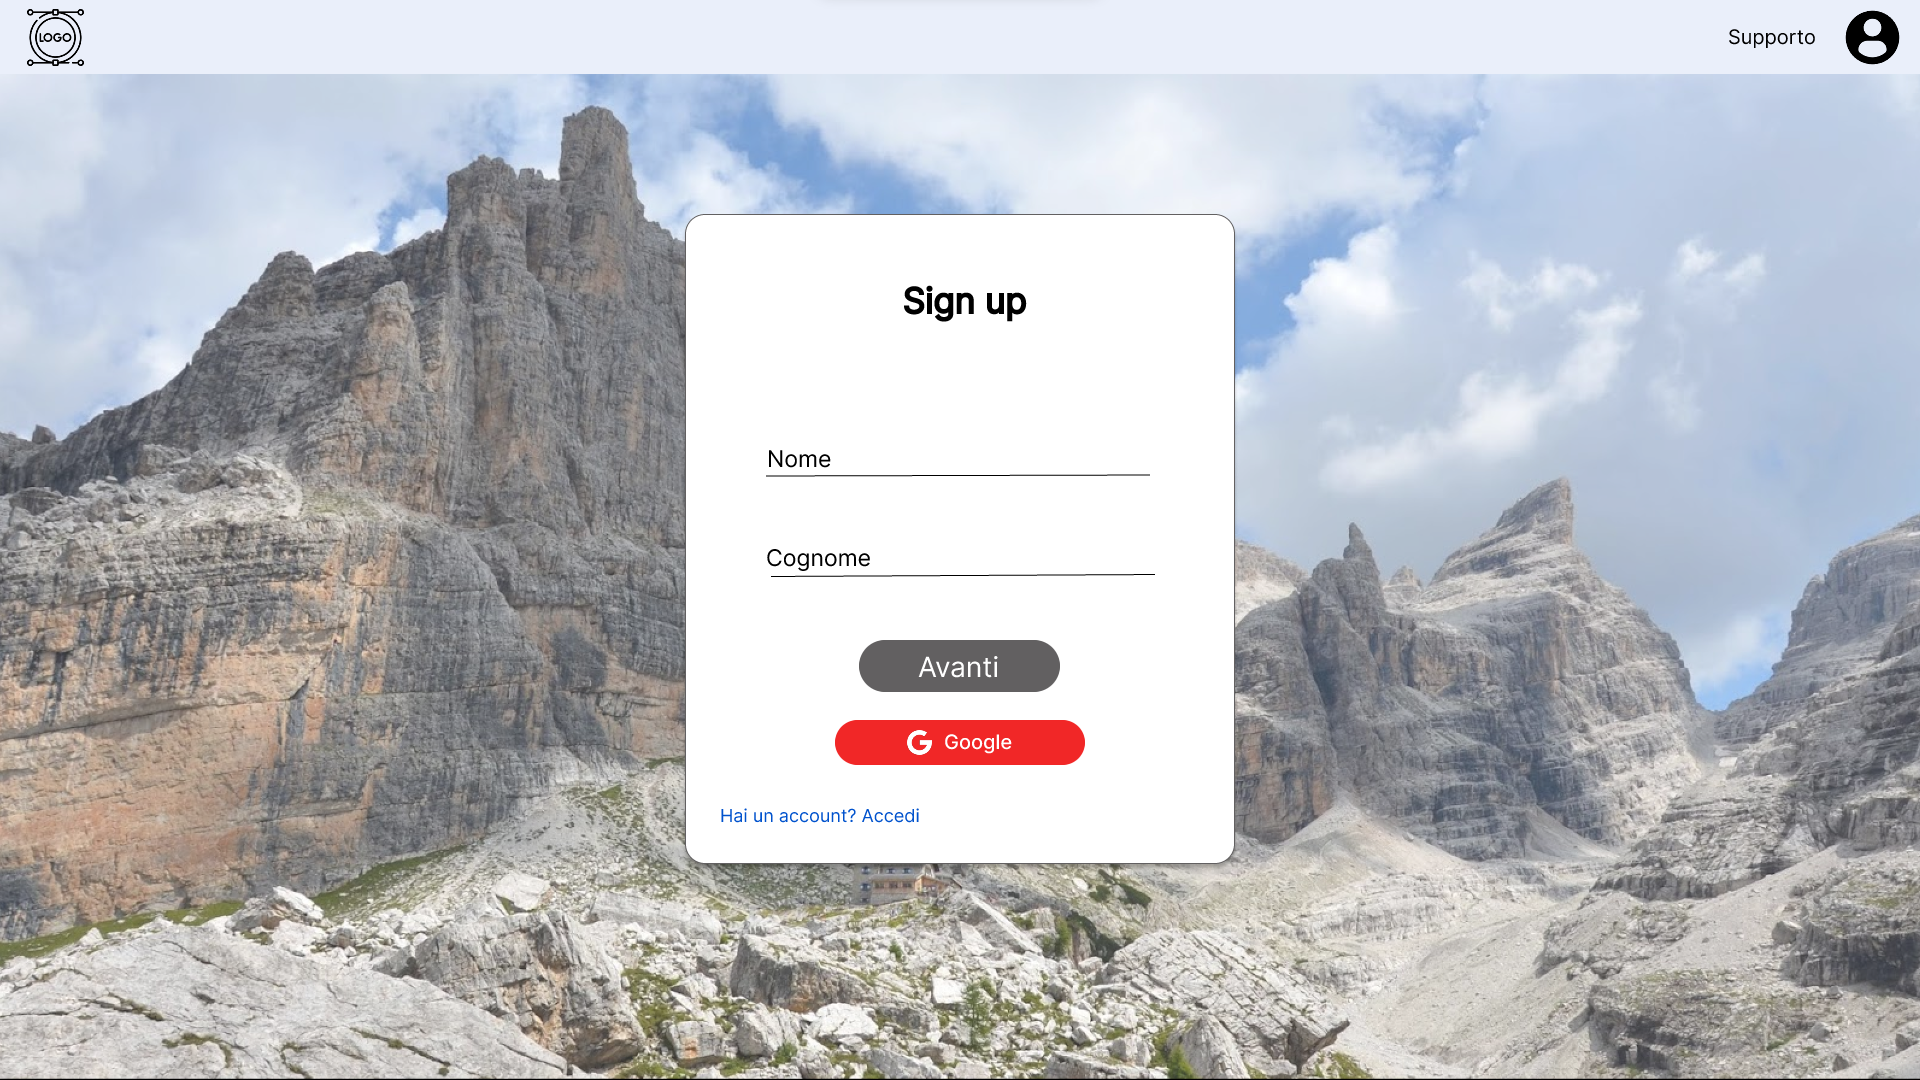
\includegraphics[width=\textwidth]{img/Sign-up 1.png} 
    \caption{Sign-up 1 pagina}
  \end{subfigure}
  \hfill % Spazio vuoto orizzontale tra le due immagini
  \begin{subfigure}{0.49\textwidth}
    \centering
    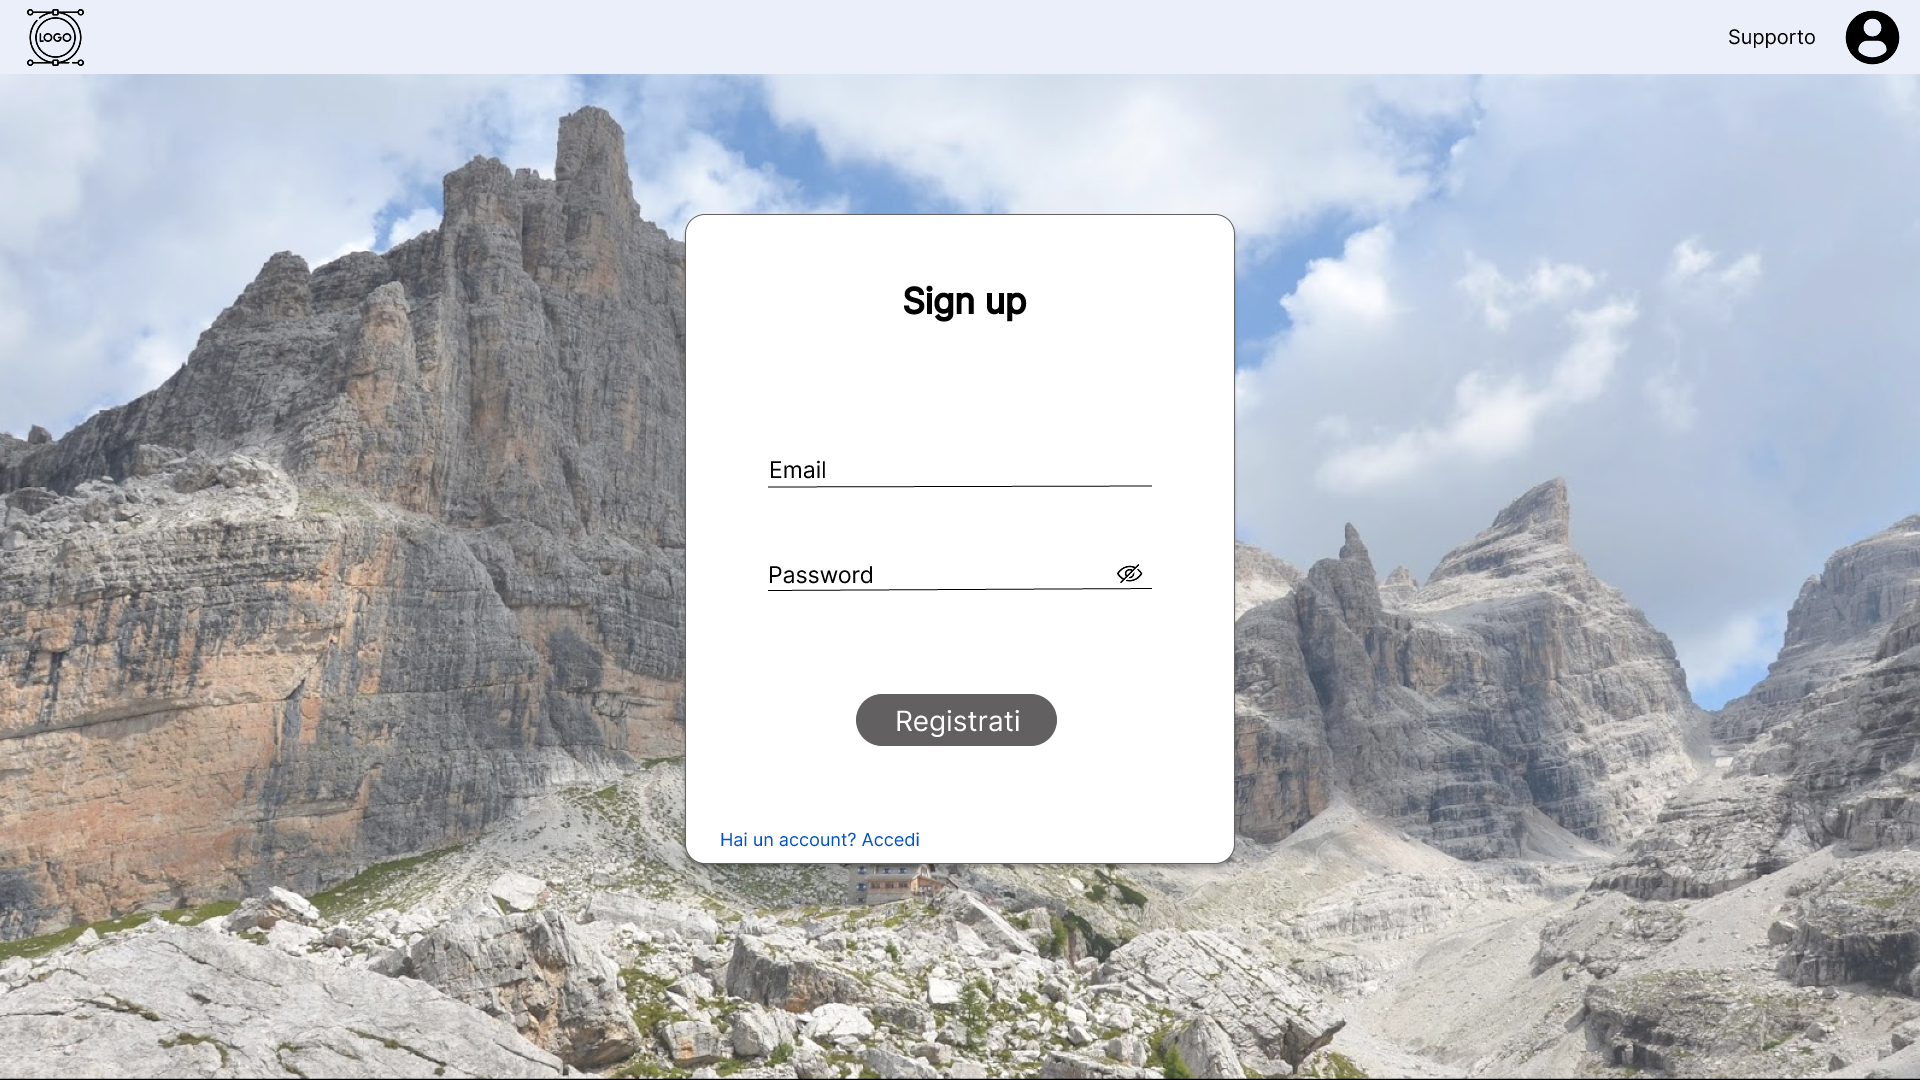
\includegraphics[width=\textwidth]{img/Sign-up 2.png} 
    \caption{Sign-up 2 pagina}
  \end{subfigure}
  \caption{Pagine di Sign-up}
\end{figure}
All'interno di queste sezioni dedicate, sarà possibile compiere il processo di registrazione (RF1) per l'ingresso di nuovi utenti nel sito web. Nel primo passo di questo processo, verrà chiesto di fornire alcune informazioni fondamentali per la creazione dell'account personale.

Nella prima sezione del modulo di registrazione, ci sarà la possibilità di inserire il nome e cognome. Questo passo iniziale è essenziale per garantire che l'account sia personalizzato e riconoscibile. Successivamente, si potrà procedere al passo successivo del processo, dove si avrà l'opzione di fornire ulteriori dettagli relativi al proprio account.

Nel secondo form, avrai la possibilità di inserire informazioni quali l'indirizzo email, che si intende associare al proprio account, e la password che si desidera utilizzare per l'accesso. L'email svolgerà un ruolo cruciale come mezzo di comunicazione e recupero dell'account, mentre la password garantirà la sicurezza dei tuoi dati personali (RNF1).



\subsection*{FE3 Sign-up page error}
\begin{figure}[htbp]
   \centering
    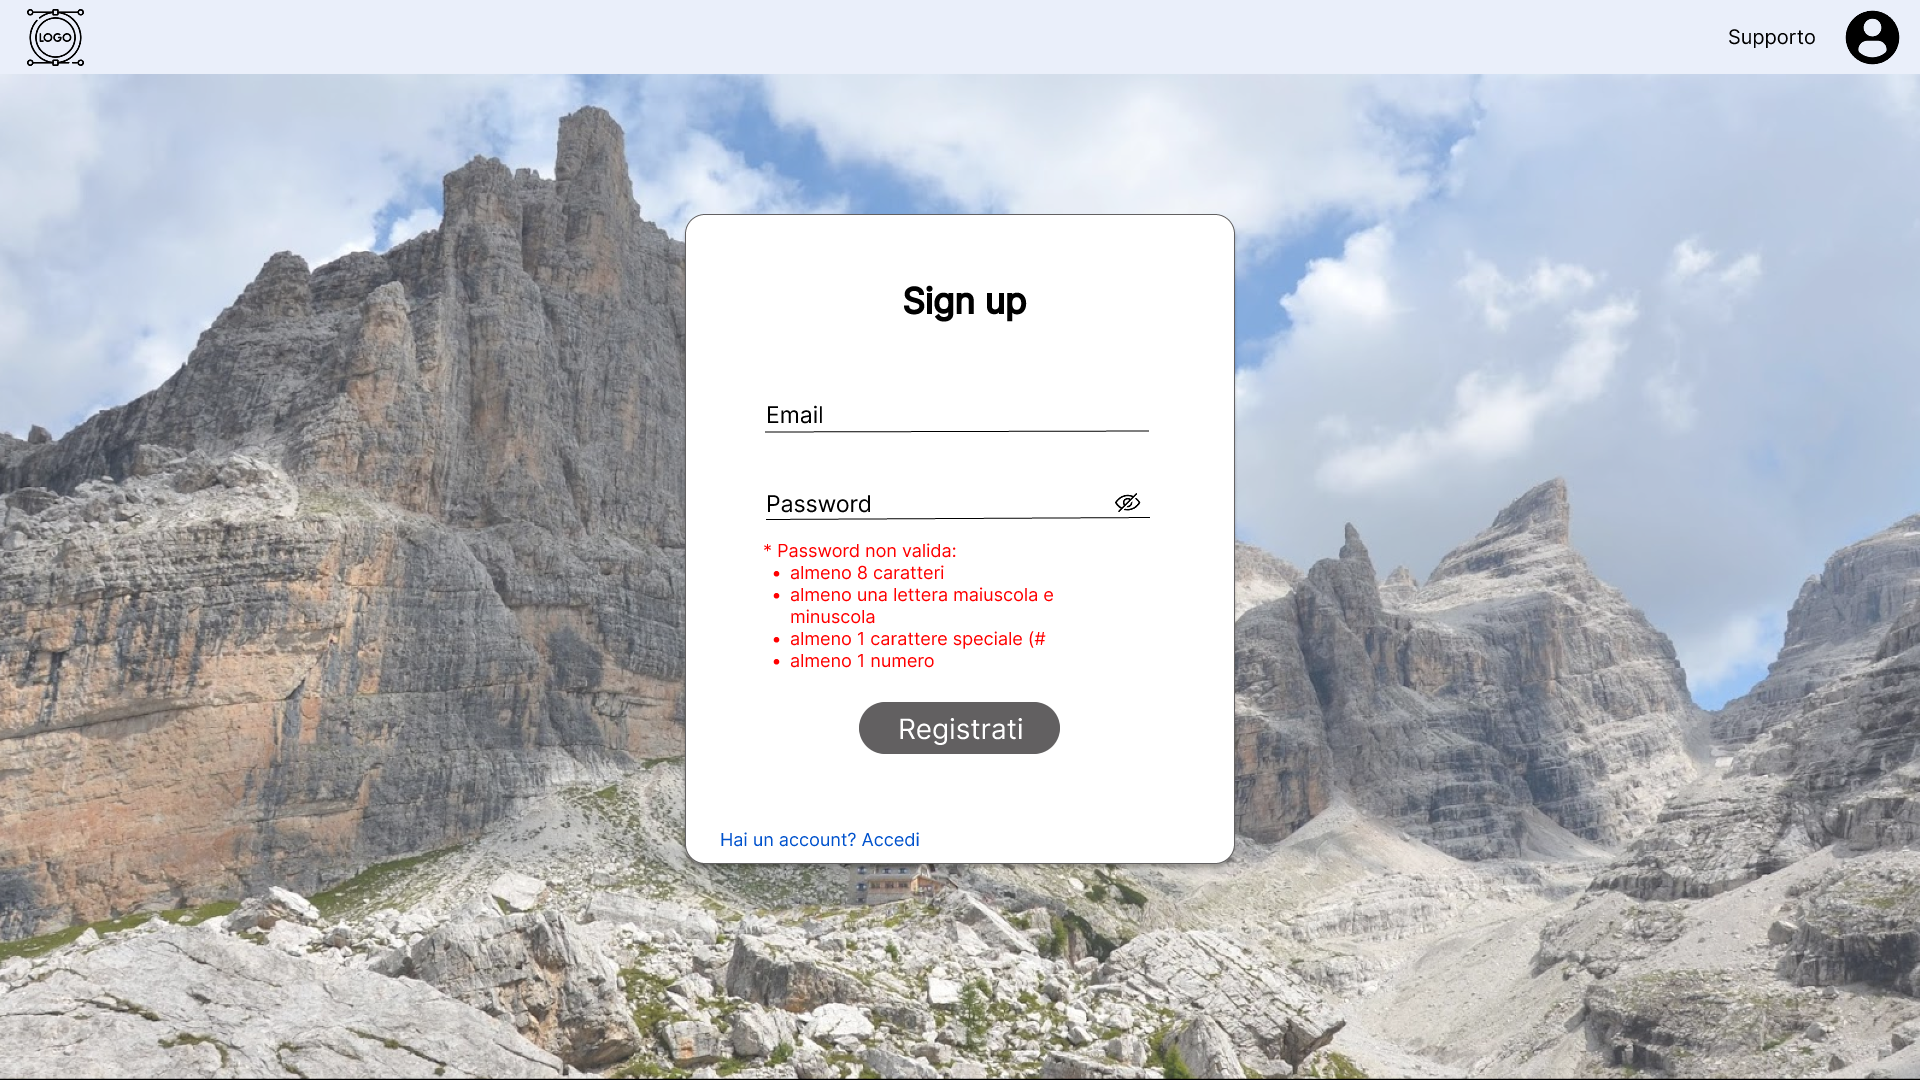
\includegraphics[width=0.6\textwidth]{img/Sign-up 3.png}
    \caption{Sign-up error}
\end{figure}
Qualora l'utente inserisca dei dati sbagliati , gli verrà mostrato un messaggio di errore per avvisarlo. (RNF1) (RF1.1)

\subsection*{FE4 Log-in page}
\begin{figure}[H]
   \centering
    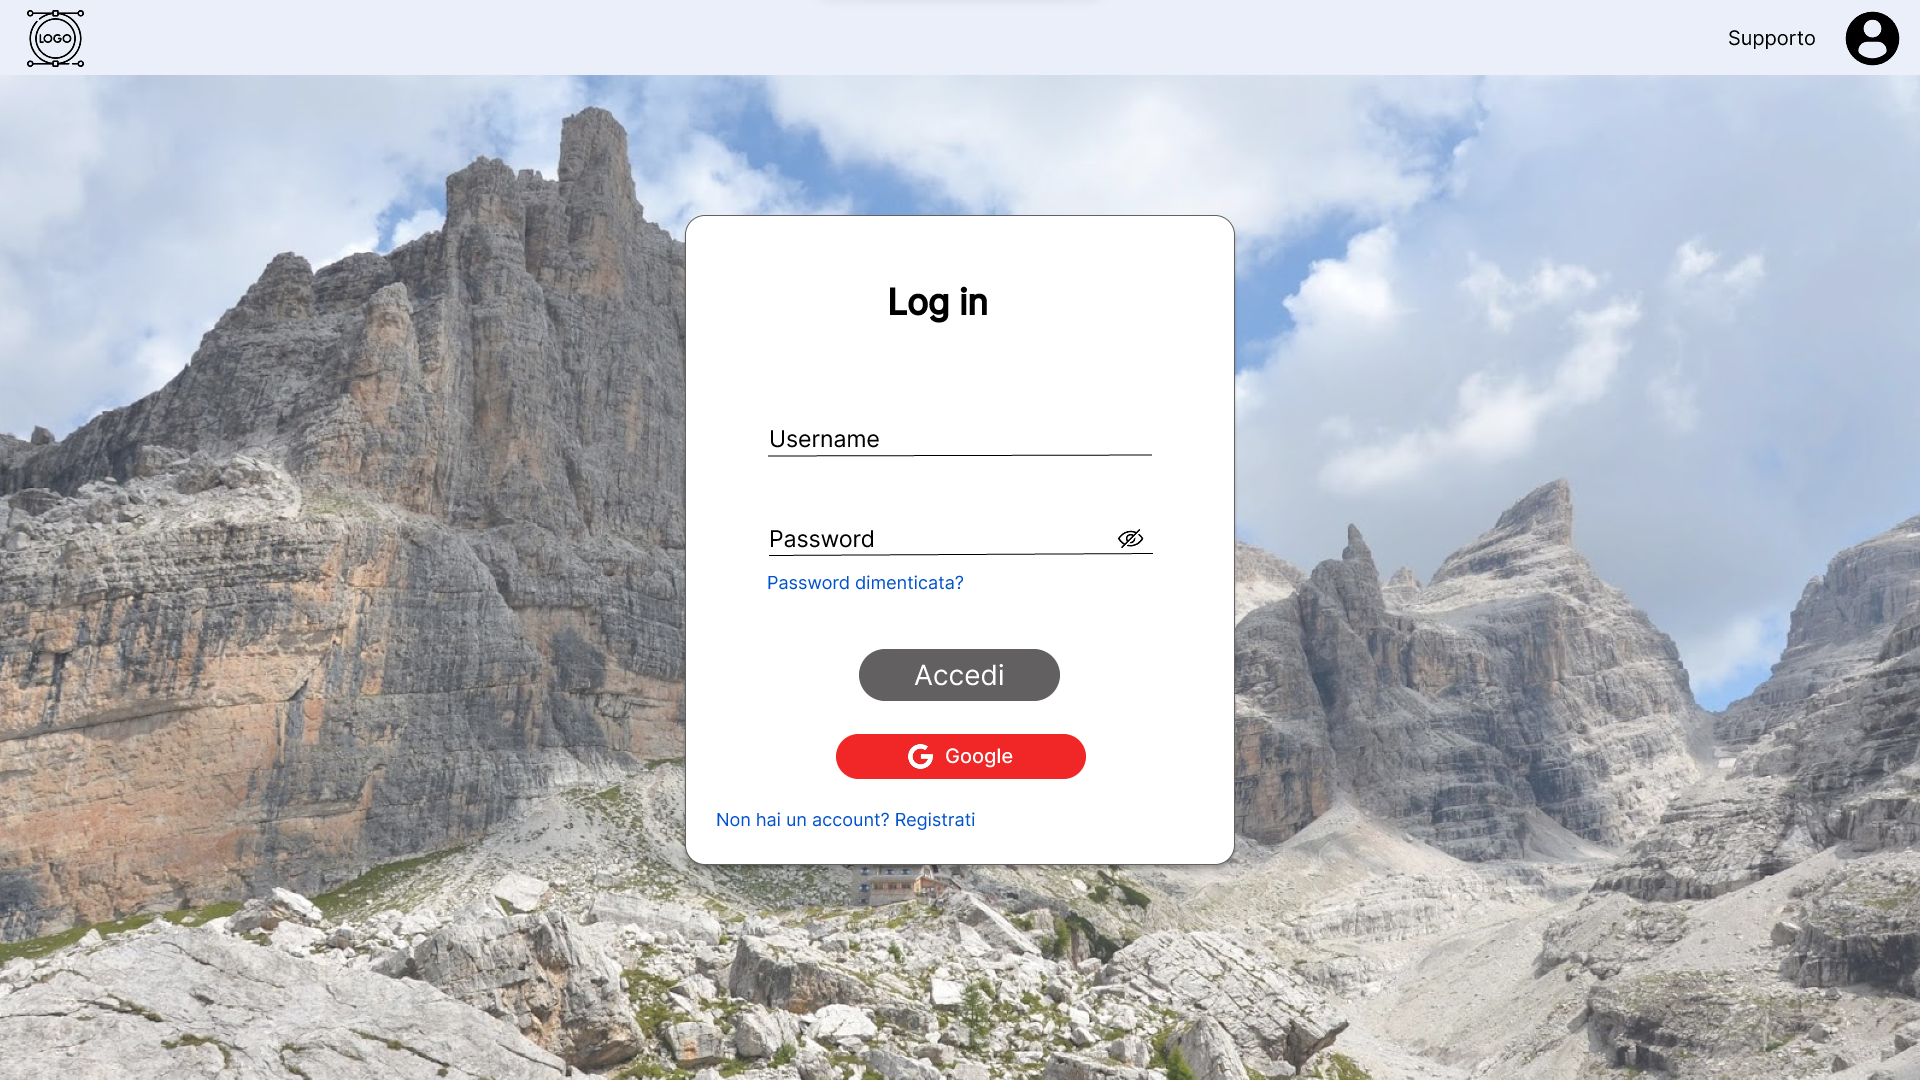
\includegraphics[width=0.6\textwidth]{img/Log-in.png}
    \caption{Pagina di log-in }
\end{figure}
Questa pagina permetterà all'utente già registrato di effettuare il login (RF2) tramite la propria email o il proprio username e la password. Una volta inseriti basterà cliccare "Accedi" per effettuare il login. Nel caso in cui l'untente non dovesse ricordarsi la password potrà, cliccando il testo: "Password dimenticata?", richiedere una nuova password che gli sarà inviata via email all'inidirizzo fornito durante la registrazione.

\subsection*{FE5 Pagina montagne}
\begin{figure}[H]
   \centering
    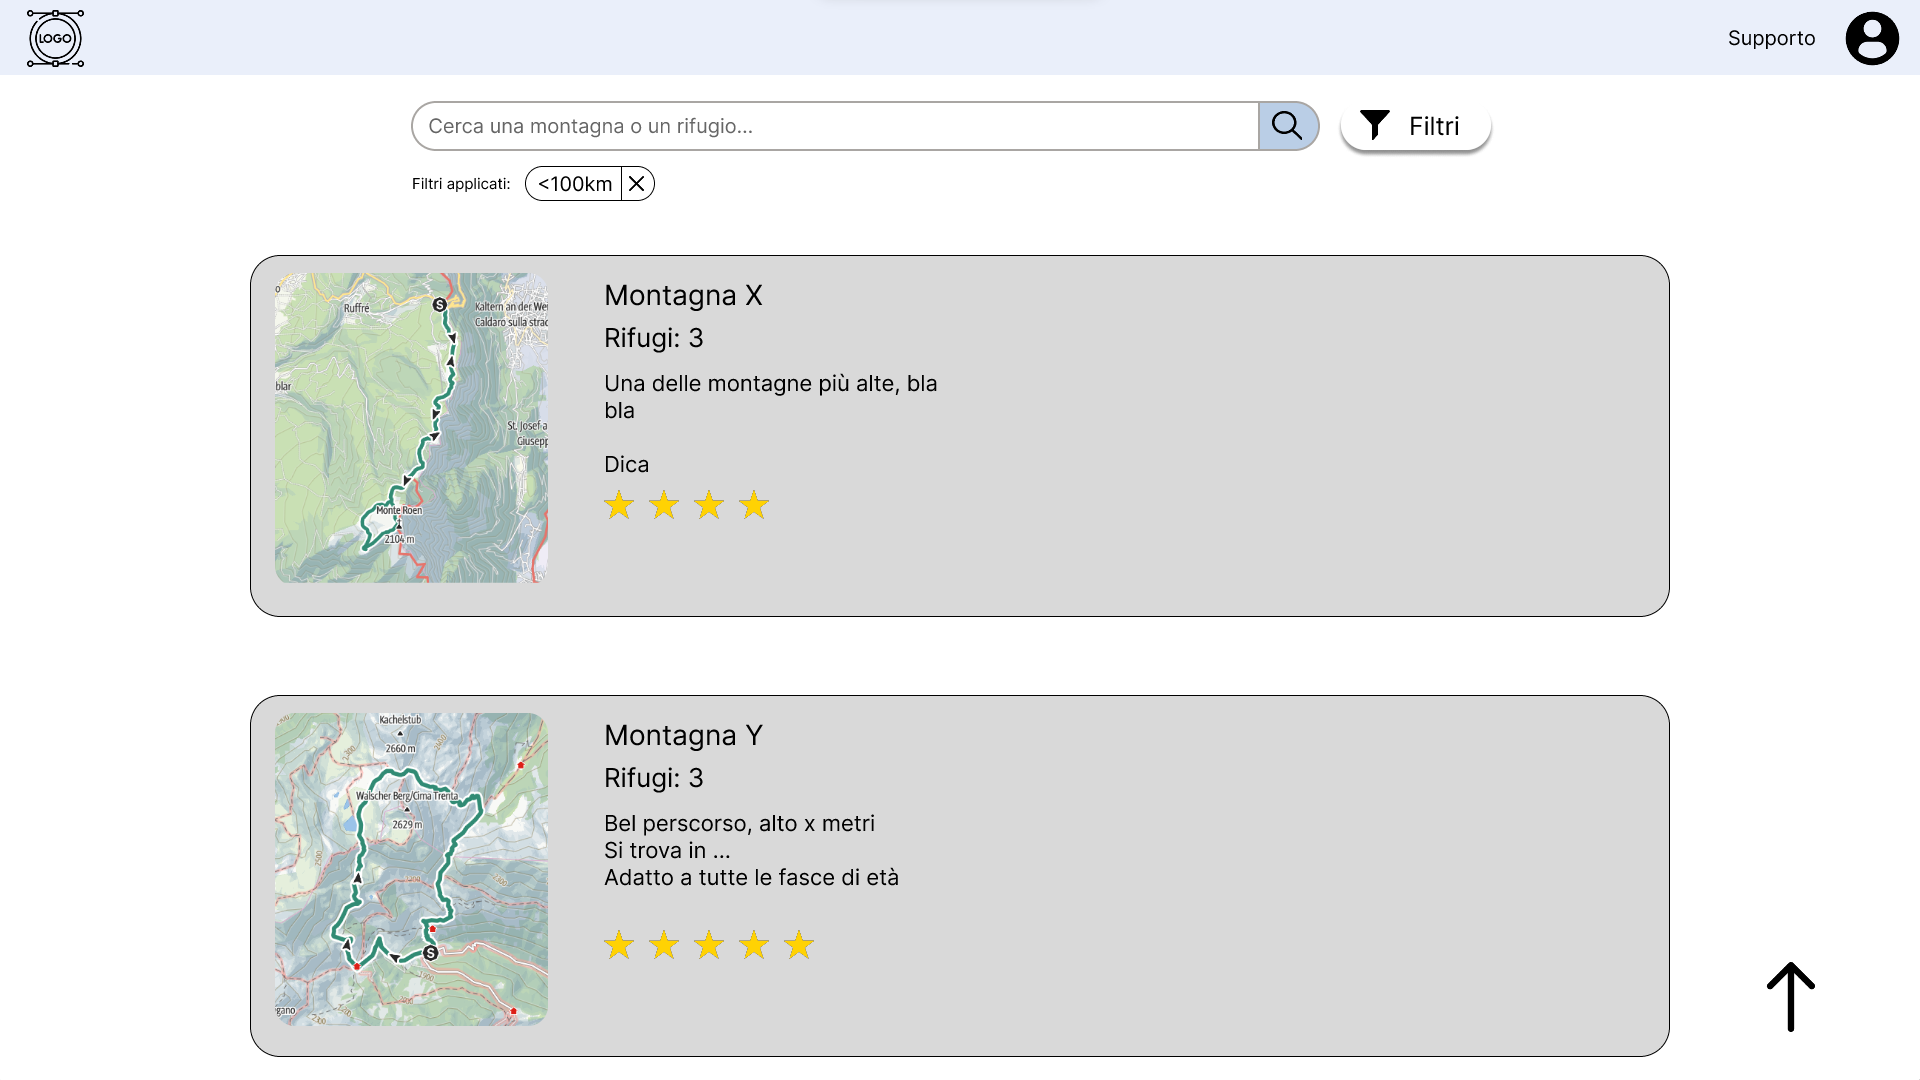
\includegraphics[width=0.6\textwidth]{img/Pagina montagne.png}
    \caption{Pagina elenco montagne}
\end{figure}
Questa pagina darà la possibilità a qualunque tipo di utente di visionare un elenco con tutte le montagne della zona. Permetterà la ricerca di un rifugio o di una montagna tramite la barra di ricerca in alto e sarà possibile applicare dei filtri per avere risultati pertinenti a quanto si deve cercare. La freccia in basso a destrà perfetterà di tornare nella homepage.

\end{document}